%%% Dateikodierung: UTF-8
%%% äöüÄÖÜß  <-- keine deutschen Umlaute hier? UTF-faehigen Editor verwenden!

%%% Magic Comments zum Setzen der korrekten Parameter in kompatiblen IDEs
% !TeX encoding = utf8
% !TeX program = pdflatex 
% !TeX spellcheck = de_DE
% !BIB program = biber

\RequirePackage[utf8]{inputenc} % bei Verw. von lualatex oder xelatex entfernen!
\RequirePackage{hgbpdfa}        % Erzeugt ein PDF/A-2b-konformes Dokument

\documentclass[bachelor,german,smartquotes,apa]{hgbthesis}
% Zulässige Optionen in [..]: 
%    Typ der Arbeit: 'diploma', 'master' (default), 'bachelor', 'internship'
%		 Zusätzlich für ein Thesis-Exposé: 'proposal' (für 'bachelor' und 'master')
%    Hauptsprache: 'german' (default), 'english'
%    Option zur Umwandlung in typografische Anführungszeichen: 'smartquotes'
%    APA Zitierstil: 'apa'
%%%-----------------------------------------------------------------------------

% Packages für Tabellen
\usepackage[table]{xcolor}
\usepackage{array}
\usepackage{multirow}
\usepackage{adjustbox}

\DocumentMetadata{lang=de}
\graphicspath{{images/}}  % Verzeichnis mit Bildern und Grafiken
\logofile{logo}           % Logo-Datei: images/logo.pdf (kein Logo: \logofile{})
\bibliography{references} % Biblatex-Literaturdatei (references.bib)

\usepackage[acronym, toc]{glossaries}
\makeglossaries
\newacronym{BERT}{BERT}{Bidirectional Encoder Representations from Transformers}
\newacronym{CNN}{CNN}{Concolutional Neural Network}
\newacronym{DONUT}{DONUT}{Document Understanding Transformer}
\newacronym{KI}{KI}{Künstliche Intelligenz}
\newacronym{LLM}{LLM}{Large Language Model}
\newacronym{LMDX}{LMDX}{Model-based Document Information Extraction} 
\newacronym{LSTM}{LSTM}{Long Short-Term Memory}
\newacronym{ML}{ML}{Machine Learning}
\newacronym{MLM}{MLM}{Masked Language Model}
\newacronym{NER}{NER}{Named Entity Recognition}
\newacronym{NLP}{NLP}{Natural Language Processing}
\newacronym{NSP}{NSP}{Next Sentence Prediction}
\newacronym{OCR}{OCR}{Optical Character Recognition}
\newacronym{POS}{POS}{Part-of-Speech}
\newacronym{RNN}{RNN}{Reccurent Neural Network}

%%%-----------------------------------------------------------------------------
\begin{document}
%%%-----------------------------------------------------------------------------

%%%-----------------------------------------------------------------------------
% Angaben für die Titelei (Titelseite, Erklärung etc.)
%%%-----------------------------------------------------------------------------

\title{Automatisierte Dokumentenverarbeitung: Implementierung und Bewertung moderner Ansätze zur Informationsextraktion}
\author{Patrick Seper}
\programname{Software Engineering}

%\programtype{Fachhochschul-Bachelorstudiengang} % auswählen/editieren
\programtype{Fachhochschul-Bachelorstudiengang}

\placeofstudy{Hagenberg}
\dateofsubmission{2025}{01}{25} % {YYYY}{MM}{DD}

\advisor{FH-Prof. DI Dr. Gabriel Kronberger} % optional

%\strictlicense % restriktive Lizenz anstatt Creative Commons (nicht empfohlen!)

%%%-----------------------------------------------------------------------------
\frontmatter                                       % Titelei (röm. Seitenzahlen)
%%%-----------------------------------------------------------------------------

\maketitle
\tableofcontents

% \chapter{Vorwort}

 % Ein Vorwort ist optional
\chapter{Kurzfassung}


		
\chapter{Abstract}


\begin{english} %switch to English language rules
%This should be a 1-page (maximum) summary of your work in English.
%und hier geht dann das Abstract weiter...
\end{english}

			

%%%-----------------------------------------------------------------------------
\mainmatter                             % Hauptteil (ab hier arab. Seitenzahlen)
%%%-----------------------------------------------------------------------------

\chapter{Einleitung}
\label{cha:einleitung}

\section{Motivation und Hintergrund}
\label{sec:motivation-und-hintergrund}

Automatisierte Dokumentenverarbeitung gewinnt in der Gewinnung strukturierter Daten zunehmend an Bedeutung. Unternehmen digitalisieren ihre Geschäftsprozesse und setzen verstärkt auf Dokumentenverarbeitungssysteme. Diese Systeme sparen Zeit und Kosten, indem sie den Bedarf an manueller Dateneingabe reduzieren und das Risiko menschlicher Fehler minimieren \parencite{PerotVincent2024LLMD}.

Die wirtschaftliche Relevanz dieser Technologie zeigt sich in der Reduzierung von Betriebskosten, der Beschleunigung von Geschäftsprozessen und der Verbesserung der Entscheidungsfindung durch zeitnahen Zugriff auf strukturierte Daten. Technologische Fortschritte in \glspl{OCR}, \glspl{NLP} und maschinellem Lernen erweitern die Möglichkeiten der automatisierten Dokumentenverarbeitung erheblich. Insbesondere \glspl{LLM} eröffnen neue Perspektiven \parencite{XuYiheng2020LPoT, TouvronHugo2023LOaE}.

Trotz dieser Fortschritte bestehen weiterhin Herausforderungen wie die Verarbeitung vielfältiger Dokumententypen, die Bewältigung von Mehrsprachigkeit und kulturellen Unterschieden in Dokumentenlayouts sowie die Gewährleistung von Datenschutz und Sicherheit.

Die Industrie wendet diese Technologien bereits praktisch an. Die Firma Multidata, selbst Hersteller eines Dokumentenverarbeitungssystems, stellt die Aufgabenstellung für diese Bachelorarbeit und unterstreicht damit die praktische Relevanz des Themas.
Das Unternehmen nutzt aktuell ein System, das auf manuell definierten Vorlagen für die Verarbeitung gleichartiger Dokumente basiert. Dieses System weist jedoch Nachteile auf. Es erfordert einen hohen manuellen Aufwand, zeigt eine geringe Anpassungsfähigkeit an sich ändernde Dokumentenlayouts und eignet sich nur eingeschränkt für bestimmte Dokumententypen.
Aufgrund dieser Limitationen strebt Multidata die Entwicklung eines Systems mit höherem Automatisierungsgrad an, das das bestehende System ersetzen soll. Abschnitt \ref{sec:analyse-des-akutell-eingesetzten-systems} erläutert die detaillierte Funktionsweise des aktuellen Systems.

Diese Bachelorarbeit verbindet akademische Forschung mit industrieller Anwendung. Sie zielt darauf ab, einen umfassenden Überblick über die aktuell im kommerziellen und wissenschaftlichen Umfeld genutzten Techniken sowie deren Leistungsfähigkeit zu bieten.

\section{Problemstellung}
\label{sec:problemstellung}

Das angestrebte Dokumentenverarbeitungssystem umfasst zwei Kernaufgaben: Dokumentenkategorisierung und Datenextraktion.

Das System muss zunächst selbstständig die Art des Dokuments bestimmen. Eine dynamische Konfiguration der verfügbaren Kategorien ermöglicht die einfache Erweiterung um neue Dokumententypen ohne umfangreiche Systemänderungen oder erneutes Modelltraining.

Anschließend extrahiert das System die für die Kategorie vorgesehenen Daten. Benutzer*innen definieren die zu extrahierenden Informationen und deren Datentyp. Das System überführt die extrahierten Daten in eine strukturierte Form zur automatisierten Weiterverarbeitung.

Da insbesondere im Umgang mit sensiblen Dokumenten der Datenschutz und die Sicherheit sehr wichtig sind, besteht die Notwendigkeit, das Dokumentenverarbeitungssystem lokal und ohne Übermittlung von Daten an externe Dienste zu betreiben. Zusätzlich soll das System plattformunabhängig sein und sowohl auf Windows- als auch auf Linux-Betriebssystemen lauffähig sein, um die Deploymentmöglichkeiten für die Kunden der Firma Multidata zu verbessern.

\section{Forschungsfrage}
\label{sec:forschungsfrage}
Diese Bachelorarbeit untersucht folgende zentrale Forschungsfrage:
Welche Methoden der automatisierten Dokumentenverarbeitung eignen sich am besten für ein flexibles, lokal betreibbares System zur Dokumentenkategorisierung und Datenextraktion, das sowohl hohe Genauigkeit als auch effiziente Laufzeit bietet?

Um diese Frage zu beantworten, ergeben sich mehrere  Teilaspekte. Zunächst gilt es, aktuelle Ansätze aus Forschung und kommerziellen Anwendungen zu untersuchen. Die Arbeit bewertet ihre Eignung für die beschriebenen Anforderungen und vergleicht ihre Genauigkeit und Laufzeit. Dabei berücksichtigt sie auch die Auswirkungen möglicher Vorverarbeitungsschritte auf die Leistung der verschiedenen Methoden.

Die Beantwortung dieser Fragen soll zu einem umfassenden Verständnis der Leistungsfähigkeit und Einsatzmöglichkeiten moderner Dokumentenverarbeitungssysteme führen und praxisrelevante Erkenntnisse für die Weiterentwicklung solcher Systeme liefern. Die Ergebnisse dieser Arbeit sollen Entwickler*innen dabei unterstützen, effizientere und genauere Dokumentenverarbeitungssysteme zu gestalten.

\section{Zielsetzung und Abgrenzung des Themas}
\label{sec:zielsetzung-und-abgrenzung}

Das Ziel der Arbeit ist es, eine geeignete Methode zur Umsetzung des beschriebenen Dokumentenverarbeitungssystems zu erarbeiten. Dazu sollen verschiedene Ansätze aus wissenschaftlichen Arbeiten verglichen werden. Zusätzlich sollen auch kommerzielle Angebote analysiert und verglichen werden, um ein ausreichend breites Bild des momentanen Stands der Technik zu erhalten.

Es soll erhoben werden, wie zuverlässig die verschiedenen Ansätze sind. Dabei soll sowohl betrachtet werden, ob die benötigten Daten gefunden werden, als auch ob das System falsche Daten erzeugt. Zusätzlich soll auch die Leistung der verschiedenen Ansätze in Bezug auf ihre empirische Laufzeit in die Vergleiche einfließen.

Als Teil dieser Analysen soll auch betrachtet werden, wie sich etwaige Schritte zur Vorverarbeitung der Dokumente auswirken. Schlussendlich soll untersucht werden, wie flexibel die verschiedenen Methoden in Bezug auf Anpassung und Veränderung sind.

Die konkrete Umsetzung im Rahmen eines zur Veröffentlichung fertigen Produktes ist nicht Teil der Zielsetzung.

\section{Methodisches Vorgehen}
\label{sec:methodisches-vorgehen}

Zuerst werden verschiedene Ansätze aus wissenschaftlichen Quellen sowie existierende Software-Bibliotheken und kommerzielle Produkte recherchiert und auf Erfüllung der definierten Anforderungen überprüft. Ansätze, die die Kriterien erfüllen, werden anschließend umgesetzt. Es werden verschiedene Tests zur Bestimmung von Genauigkeit und empirischer Laufzeit durchgeführt. Dazu werden sowohl öffentlich verfügbare Datensätze als auch von Multidata zur Verfügung gestellte Datensätze genutzt. Die Ergebnisse werden anschließend grafisch aufbereitet und verglichen. Abschließend werden verschiedene Verbesserungsansätze, wie unterschiedliche Methoden zum Vorbereiten der Dokumente, implementiert und ihre Auswirkungen gemessen und dokumentiert.

Unterstützend zur Verbesserung der Formulierung, sowie zur Rechtschreib- und Grammatikprüfung wird das \gls{LLM} Claud 3.5 Sonnet \parencite{anthropic_claude} verwendet.
\chapter{Technische Grundlagen}
\label{cha:Technische Grundlagen}

Dieses Kapitel gibt einen Überblick über die wichtigsten technischen Konzepte und Methoden, die für das Verständnis moderner Dokumentenverarbeitungssysteme grundlegend sind. Dabei werden sowohl grundlegende Konzepte als auch Metriken zur Messung des Erfolgs bearbeitet. 

\section{Optical Character Recognition (OCR)}
\label{sec:optical-character-recognition-ocr}

\gls{OCR} ist eine Schlüsseltechnologie bei der Verarbeitung von visuellen Dokumenten. Sie erfüllt die Aufgabe, Bilder von gedrucktem oder handgeschriebenem Text in maschinenlesbaren Text umzuwandeln \cite{MoriS.1992HroO}.
Auch wenn \gls{OCR} für Optical Character Recognition steht, erkennen viele der gängigen Systeme in Wahrheit Zeichenblöcke oder ganze Wörter \cite{BorovikovEugene2014Asom}.
Es gibt eine Vielzahl an verschiedenen \gls{OCR} Methoden, von denen einige Segmentierung, also die Zuteilung jedes Pixels zu einer Kategorie, verwenden und andere nicht \cite{BorovikovEugene2014Asom}. Die meisten modernen \gls{OCR}-Systeme bestehen dabei typischerweise aus zwei essenziellen Teilen \cite{BorovikovEugene2014Asom}:

\begin{enumerate}
    \item Feature Extractor: Basierend auf einem Bild eines Elements extrahiert dieser die charakteristischen Merkmale (Deskriptoren) des Elements. Diese abgeleiteten Merkmale dienen als Eingabe für den Classifier.
    \item Classifier: Dieser bestimmt anhand der extrahierten Merkmale das (wahrscheinlichste) bekannte Element. Zusätzlich liefert der Classifier einen Konfidenzwert, der angibt, wie sicher die Erkennung des Elements ist.
\end{enumerate}

Diese grundlegende Struktur bildet die Basis für verschiedene klassische und moderne Methoden der optischen Zeichenerkennung \cite{BorovikovEugene2014Asom}:

\begin{itemize}
\item Template Matching: Vergleicht Eingabezeichen pixelweise mit bekannten Vorlagen und wählt die ähnlichste aus.
\item Strukturelle Klassifikation: Nutzt strukturelle Merkmale wie Striche, Löcher oder Ecken und wendet regelbasierte Systeme an.
\end{itemize}

Dabei ist zu beachten, dass es auch leichte Abweichungen und hybride Varianten von diesen Techniken gibt \cite{BorovikovEugene2014Asom}. Viele moderne \gls{OCR}-Systeme verwenden mathematische Funktionen, die darauf abzielen, eine Metrik der Abweichung von einer Vorlage zu minimieren; Beispiele dafür sind \cite{BorovikovEugene2014Asom}:

\begin{itemize}
    \item Diskriminanzfunktionen: Verwenden Hyperebenen im mehrdimensionalen Merkmalsraum zur Trennung von Zeichenklassen.
    \item Bayes-Klassifikatoren: Minimieren Fehlklassifikationen mittels Wahrscheinlichkeitstheorie.
    \item Künstliche Neuronale Netze (KNN): Lernen komplexe Klassifikationsabbildungen durch Fehlerrückführung und Optimierungstechniken.
\end{itemize}

\subsection{Tesseract OCR}
\label{subsec:tesseract-ocr}
Das für die im Rahmen dieser Bachelorarbeit implementierten Prototypen verwendete \gls{OCR}-System heißt Tesseract \gls{OCR}. Dabei handelt es sich um ein ursprünglich von Hewlett Packard entwickeltes \gls{OCR}-System, welches seit 2005 als Open-Source-Software verfügbar ist \cite{SmithR_2007_AOot}. Tesseract basiert auf \gls{LSTM} neuronalen Netzen, welches über 100 Sprachen und über 35 Schriftsysteme unterstützt \cite{tesseract_ocr_user_manual}. 

\subsubsection{Architektur und Funktionsweise}
\label{subsubsec:architektur-und-funktionsweise}
Tesseract folgt einem traditionellen Pipeline-Ansatz für die Texterkennung, wobei einige Schritte zur Zeit ihrer Entwicklung ungewöhnlich waren \cite{SmithR_2007_AOot}. Der Prozess beginnt mit einer Analyse verbundener Komponenten, bei der die Umrisse der Komponenten gespeichert werden. Diese Methode ermöglicht es Tesseract, sowohl schwarzen Text auf weißem Hintergrund als auch umgekehrt zu erkennen \cite{SmithR_2007_AOot}.

\subsubsection{Zeilenfindung und Basislinienanpassung}
\label{subsubsec:zeilenfindung-und-basislinienanpassung}
Ein wichtiger Aspekt von Tesseract ist der Algorithmus zur Zeilenfindung, der es ermöglicht, schiefe Seiten ohne vorherige Entzerrung zu erkennen. Dies verhindert einen Qualitätsverlust des Bildes \cite{SmithR_2007_AOot}. Nach der Zeilenerkennung werden die Basislinien mittels präzise angepasst, was Tesseract befähigt, auch mit gekrümmten Basislinien umzugehen, was ein häufiges Problem ein häufiges Problem beim Scannen von Büchern ist \cite{SmithR_2007_AOot}.

\subsubsection{Zeichenerkennung und Klassifizierung}
\label{subsubsec:zeichenerkennung-und-klassifizierung}
Tesseract verwendet einen zweistufigen Klassifizierungsprozess, um sich auf die etwaige Schriftart sowie mögliche Artefakte anzupassen \cite{SmithR_2007_AOot}:

Zuerst erstellt ein schneller Vorfilter eine Liste möglicher Zeichenklassen. Dann wird für diese Auswahl eine genauere Ähnlichkeitsberechnung durchgeführt. Diese Methode ist effizient und genau zugleich. 

Zusätzlich nutzt Tesseract einen adaptiven Klassifizierer. Dieser lernt während des Erkennungsvorgangs dazu und passt sich so an die spezifischen Eigenschaften des aktuellen Dokuments an. Er verwendet die gleichen Grundlagen wie der Hauptklassifizierer, normalisiert die Eingabedaten aber anders, was die Erkennung von Groß- und Kleinbuchstaben verbessert und die Störungsanfälligkeit verringert \cite{SmithR_2007_AOot}.

Diese Kombination aus effizientem zweistufigem Prozess und anpassungsfähigem Lernen ermöglicht Tesseract eine genaue Texterkennung in verschiedenen Dokumenttypen und Schriftstilen.

\section{Grundlagen des Machine Learning}
\label{sec:machine-learning-grundlagen}
 \gls{ML} ist ein Teilbereich der Informatik, der sich mit Algorithmen und Techniken zur Automatisierung komplexer Problemlösungen befasst \cite{RebalaGopinath2019AItM}. \gls{ML}-Algorithmen lernen aus Daten, ohne explizit programmiert zu werden \cite{RebalaGopinath2019AItM}. Der Unterschied zur konventionellen Programmierung liegt dabei darin, dass \gls{ML} selbständig Regeln aus Beispieldaten erstellt, statt einem definierten Regelwerk zu folgen.

Dabei werden verschiedene Arten von Lernvorgängen unterschieden \cite{RebalaGopinath2019AItM, jordan2015machine}:
\begin{itemize}
    \item Überwachtes Lernen (Supervised Learning): Der Algorithmus lernt anhand von gelabelten Trainingsdaten. Beispiele sind Klassifikations- und Regressionsaufgaben.
    \item Unüberwachtes Lernen (Unsupervised Learning): Der Algorithmus findet Muster in ungelabelten Daten, z.B. beim Clustering.
    \item Semi-überwachtes Lernen (Semi-supervised Learning): Eine Kombination aus gelabelten und ungelabelten Daten wird verwendet. Dieser Fall wird häufig bei Mangel von gelabelten Daten angewandt.
    \item Verstärkendes Lernen (Reinforcement Learning): Der Algorithmus lernt durch Interaktion mit einer Umgebung und erhält Belohnungen für bestimmte Aktionen.
\end{itemize}

Die großen Fortschritte im Bereich des Machine Learning in den letzten Jahren sind auf verschiedene Faktoren zurückzuführen, darunter die Verfügbarkeit großer Datenmengen, die Zunahme der Rechenleistung und verbesserte Algorithmen für große Datensätze \cite{jordan2015machine}.
Im Rahmen von \gls{ML} gibt es verschiedene Unterarten, welche in den folgenden Absätzen besprochen werden, einen Überblick darüber bietet die Abbildung \ref{fig:ml-hierarchy}.

\begin{figure}[h]
	\centering
	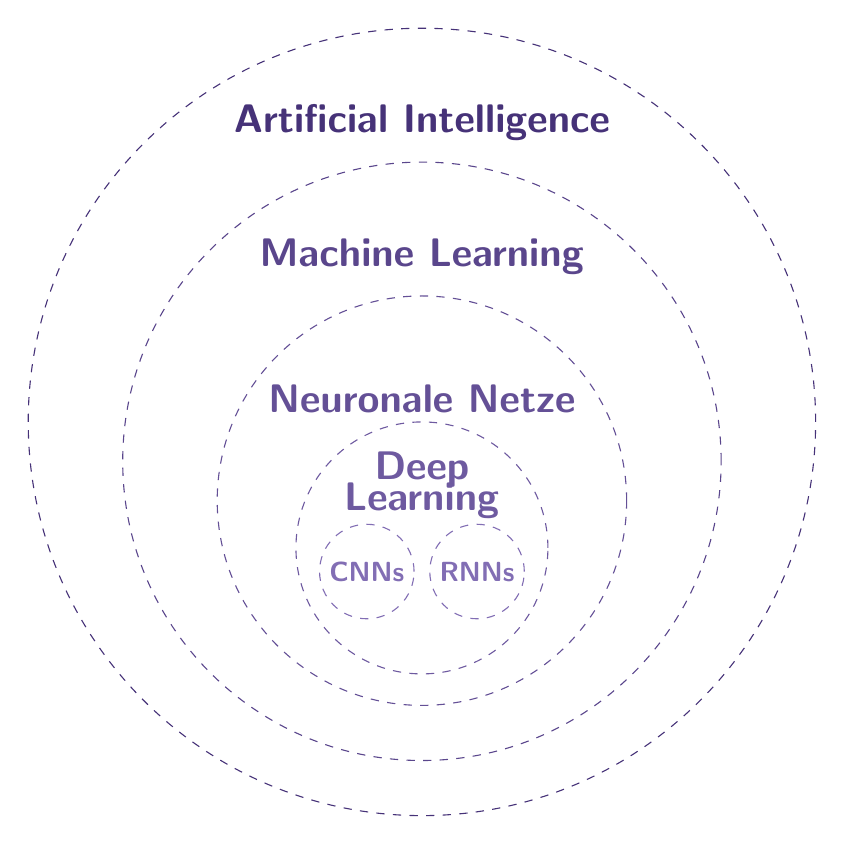
\begin{tikzpicture}[font=\sffamily]
		% Define colors
		\definecolor{outercolor}{RGB}{70,50,120}
		\definecolor{middlecolor}{RGB}{90,70,140}
		\definecolor{innermiddlecolor}{RGB}{100,80,150}
		\definecolor{innercolor}{RGB}{110,90,160}
		\definecolor{innermostcolor}{RGB}{130,110,180}
		% Outer circle (Artificial Intelligence)
		\draw[dashed, outercolor] (0,0) circle (5cm);
		\node[outercolor] at (0,3.8) {\Large\textbf{Artificial Intelligence}};
		% Middle circle (Machine Learning)
		\draw[dashed, middlecolor] (0,-0.5) circle (3.8cm);
		\node[middlecolor] at (0, 2.1) {\Large\textbf{Machine Learning}};
		% Inner-middle circle (Neuronale Netze)
		\draw[dashed, innermiddlecolor] (0,-1) circle (2.6cm);
		\node[innermiddlecolor] at (0,0.3) {\Large\textbf{Neuronale Netze}};
		% Inner circle (Deep Learning)
		\draw[dashed, innercolor] (0,-1.6) circle (1.6cm);
		\node[innercolor] at (0,-0.6) {\Large\textbf{Deep}};
		\node[innercolor] at (0,-1) {\Large\textbf{Learning}};
		% Innermost circles (CNNs and RNNs)
		\draw[dashed, innermostcolor] (-0.7,-1.9) circle (0.6cm);
		\node[innermostcolor] at (-0.7,-1.9) {\textbf{CNNs}};
		\draw[dashed, innermostcolor] (0.7,-1.9) circle (0.6cm);
		\node[innermostcolor] at (0.7,-1.9) {\textbf{RNNs}};
	\end{tikzpicture}
	\caption{Zusammenhang von Machine Learning, neuronalen Netzen, Deep Learning, \glspl{CNN} und \glspl{RNN}}
	\label{fig:ml-hierarchy}
\end{figure}

\subsection{Neuronale Netze}
\label{subsec:neuronale-netze}
Neuronale Netze sind eine Klasse von \gls{ML}-Modellen, die von der Funktionsweise des menschlichen Gehirns inspiriert sind \cite{RebalaGopinath2019AItM}. Sie bestehen aus miteinander verbundenen Neuronen, die in Schichten angeordnet sind:
\begin{itemize}
    \item Eingabeschicht (Input Layer): Nimmt die Eingabedaten auf
    \item Versteckte Schichten (Hidden Layer): Verarbeiten die Informationen
    \item Ausgabeschicht (Output Layer): Liefert das Ergebnis
\end{itemize}

Die Verbindungen zwischen den Neuronen haben Gewichte, die während des Trainings angepasst werden. Durch nichtlineare Aktivierungsfunktionen können neuronale Netze komplexe Zusammenhänge modellieren.

\subsubsection{Deep Learning}
\label{subsec:deep-learning}
Deep learning bezeichnet neuronale Netze die über viele versteckte Schichten verfügen \cite{RebalaGopinath2019AItM}, wodurch hierarchische Merkmale aus den Daten extrahiert werden können. Die Entwicklung von Deep Learning Algorithem führte in den letzten Jahren zu großen Fortschritten im Bereichen wie Bilderkennung, Sprachverarbeitung, Robotik oder auch \gls{OCR} \cite{jordan2015machine}.

Wichtige Konzepte im Deep Learning sind:
\begin{itemize}
	\item Backpropagation: Algorithmus zum effizienten Training durch Berechnung der Gradienten \cite{RebalaGopinath2019AItM}
	\item Regularisierung: Techniken zur Vermeidung von Overfitting \cite{jordan2015machine}
	\item Transfer Learning: Übertragung gelernter Merkmale auf neue Aufgaben \cite{jordan2015machine}
\end{itemize}


\subsubsection{Convolutional Neural Networks (CNNs)}
\label{subsubsec:cnn}
CNNs sind eine spezielle Art von neuronalen Netzen, die besonders für die Verarbeitung von Bilddaten geeignet sind \cite{RebalaGopinath2019AItM}. Sie nutzen Faltungsoperationen (Convolutions), um lokale Muster in den Eingabedaten zu erkennen. Im Kontext von \glspl{CNN} gibt es verschiedene gängige Ebenentypen \cite{RebalaGopinath2019AItM}:

\begin{itemize}
	\item Convolutional Layer: Anwendung von Filtern (Kernel) zur Merkmalserkennung
	\item ReLU (Rectified Linear Unit): nach einer Faltungsschicht wird häufig eine ReLU Funktion angewandt um die Komplexität des Modells zu reduzieren; dazu werden nichtlineare Merkmale eingeführt und negative Werte auf Null gesetzt
	\item Pooling Layer: Reduzierung der räumlichen Dimensionen
	\item Fully Connected Layer: verbinden jedes Neuron mit allen Neuronen der vorhergehenden Schicht; führen Klassifikation basierend auf extrahierten Merkmalen durch
\end{itemize}

CNNs haben sich als sehr leistungsfähig für Aufgaben wie Objekterkennung, Gesichtserkennung und autonomes Fahren erwiesen \cite{RebalaGopinath2019AItM}.

\section{Natural Language Processing (NLP)}
\label{sec:nlp}
\gls{NLP} befasst sich mit dem Verstehen und der Interpretation von menschlicher
Sprachen, gesprochen oder geschrieben, mit Hilfe maschineller Verarbeitung \cite{RebalaGopinath2019AItM}. \gls{NLP} ist nützlich für eine Vielzahl von
Anwendungen wie Spracherkennung, Sprachübersetzungen, Zusammenfassungen,
Fragebeantwortung, Spracherzeugung und Suchanwendungen.

\subsection{Tokenisierung}
\label{subsec:tokenisierung}
Die Tokenisierung ist ein fundamentaler Schritt in der Verarbeitung natürlicher Sprache. Hierbei wird ein Text in einzelne Einheiten, sogenannte Token, zerlegt \cite{RebalaGopinath2019AItM}. In den meisten Fällen entsprechen diese Token einzelnen Wörtern, können aber auch Satzzeichen oder andere bedeutungstragende Elemente umfassen \cite{RebalaGopinath2019AItM}. Ein einfacher Ansatz in Englischen Texten ist dazu beispielsweise den Text bei Leerzeichen zu trennen.

\subsection{Part-of-Speech Tagging}
\label{subsec:pos-tagging}
Im \gls{POS}-Tagging-Schritt wird jedes Wort in einem Text einer grammatikalischen Katgorie wie zum Beispiel Nomen, Verb, Adjektiv et cetera zugeordnet \cite{RebalaGopinath2019AItM}. Dieser Schritt ist wichtig, da die grammatikalische Funktion einens Wortes oft entscheidend für seine Bedeutung im Kontext ist.

\subsection{Named Entity Recognition}
\label{subsec:ner}
\gls{NER} ist eine zentrale Aufgabe im \gls{NLP}, bei der es darum geht, benannte Entitäten in einem Text zu identifizieren und zu klassifizieren \cite{nadeau2007survey}. Benannte Entitäten sind typischerweise Eigennamen von Personen, Organisationen, Orten, aber auch Zeitangaben, Währungen und andere spezifische Bezeichnungen.

\gls{NER}-Systeme müssen in der Lage sein, mehrdeutige Begriffe korrekt zu interpretieren. Beispielsweise kann "Tesla" je nach Kontext als Personenname, Unternehmensname oder als Einheit für magnetische Flussdichte verstanden werden \cite{RebalaGopinath2019AItM}.

Frühe \gls{NER}-Systeme basierten hauptsächlich auf manuell erstellten Regeln und Wörterbüchern \cite{nadeau2007survey}. Moderne Ansätze nutzen jedoch zunehmend maschinelle Lernverfahren, insbesondere überwachtes Lernen. Dabei werden Modelle auf großen, annotierten Texten trainiert, um Muster und Kontexte zu erkennen, die auf benannte Entitäten hindeuten \cite{nadeau2007survey}.
Diese beiden Ansätze können auch kombiniert werden, um die Flexibilität des maschinellen Lernens mit domänenspezifischen Wissen zu kombinieren \cite{nadeau2007survey}. Dies verbessert die Genauigkeit und hat sich als besonders effektiv erwiesen. Die Leistungsfähigkeit wird dabei typischerweise anhand von Präzision und Recall gemessen.

\section{Transformer-Architekturen und Large Language Models}
\label{sec:transformers-llms}

\subsection{Transformer-Architektur}
\label{subsec:transformer-architecture}

Die Transformer-Architektur, erstmals von \textcite{VaswaniAshish2023AIAY}. vorgestellt, revolutionierte das Feld des maschinellen Lernens für natürliche Sprache. Im Gegensatz zu früheren rekurrenten oder faltungsbasierten Modellen basiert der Transformer vollständig auf Aufmerksamkeitsmechanismen (Attention), was eine effizientere Verarbeitung langer Sequenzen ermöglicht.

Kernelemente der Transformer-Architektur sind \cite{VaswaniAshish2023AIAY}:
\begin{itemize}
	\item Multi-Head Attention: Ermöglicht dem Modell, verschiedene Aspekte der Eingabe parallel zu berücksichtigen.
	\item Positionscodierung: Fügt Informationen über die Reihenfolge der Tokens hinzu, da die Attention-Mechanismen selbst keine Reihenfolge berücksichtigen.
	\item Feed-Forward-Netzwerke: Verarbeiten die Ausgaben der Attention-Layer weiter.
	\item Residuale Verbindungen und Layer-Normalisierung: Verbessern den Informationsfluss und stabilisieren das Training.
\end{itemize}

Die Transformer-Architektur hat sich aufgrund ihrer Skalierbarkeit und Effizienz als Grundlage für viele moderne Sprachmodelle etabliert \cite{VaswaniAshish2023AIAY}.

\subsection{BERT und verwandte Modelle}
\label{subsec:bert}

Die von \textcite{DevlinJacob2019BPoD} vorgestellte \gls{BERT}-Technologie war ein weiterer bedeutender Fortschritt in der Anwendung von Transformer-Architekturen. BERT verwendet eine bidirektionale Vortrainingsmethode, die es dem Modell ermöglicht, Kontext aus beiden Richtungen zu berücksichtigen \cite{DevlinJacob2019BPoD}.

Wichtige Aspekte dieses Trainingsprozesses sind \cite{DevlinJacob2019BPoD}:
\begin{itemize}
	\item Masked Language Model (MLM): Trainiert das Modell, maskierte Wörter in einem Satz vorherzusagen.
	\item Next Sentence Prediction (NSP): Trainiert das Modell, die Beziehung zwischen Satzpaaren zu verstehen.
\end{itemize}
 \gls{BERT}\cite{DevlinJacob2019BPoD} sowie Varianten wie ALBERT\cite{LanZhenzhong2019AALB} oder RoBERTa\cite{liu2019robertarobustlyoptimizedbert} haben zu signifikanten Verbesserungen in vielen natürlichen Sprachverarbeitungsaufgaben geführt.

\subsection{Large Language Models (LLMs)}
\label{subsec:llms}

\subsubsection{LLAMA}
\label{subsubsec:LLAMA}

\subsection{Herausforderungen und Einschränkungen}
\label{subsec:llm-challenges}

\section{Evaluation und Metriken}
\label{sec:evaluation-metrics}

\subsection{Precision, Recall und F1-Score}
\label{subsec:precision-recall-f1}

\subsection{Micro-F1 und Macro-F1}
\label{subsec:micro-macro-f1}

\section{Lernparadigmen und Aufgabenkategorien}
\label{sec:lernparadigmen-aufgabenkategorien}

\subsection{Transfer Learning}
\label{subsec:transfer-learning}

\subsection{Few-Shot Learning}
\label{subsec:few-shot-learning}

\subsection{Zero-Shot Learning}
\label{subsec:zero-shot-learning}

\subsection{Meta-Learning}
\label{subsec:meta-learning}

\subsection{Multitask Learning}
\label{subsec:multitask-learning}

\chapter{Problemanalyse und Stand der Technik}
\label{cha:problemanalyse-stand-der-technik}

Dieses Kapitel beleuchtet die Problemstellung detailliert. Es analysiert sowohl die aktuell eingesetzte Lösung als auch gängige Methoden in Forschung und kommerziellen Anwendungen.

\section{Analyse des aktuell eingesetzten Systems}
\label{sec:analyse-des-akutell-eingesetzten-systems}

\subsection{Architektur und Funktionsweise}
\label{subsec:architektur-und-funktionsweise}

Das bestehende System nutzt Zonal-\gls{OCR} zur Dokumentenverarbeitung \cite{multidata_help}. 
Vorlagen mit Bounding Boxes definieren die zu erfassenden Zonen. 
Nutzer*innen erstellen für jedes Dokumentenlayout eine Vorlage mit vier Hauptkomponenten:

\begin{itemize}
	\item Suchfelder: Diese legen Position, Bezeichnung und Typ der zu extrahierenden Daten fest.
	\item Identifikationsmerkmale: Sie bestimmen die Position und den spezifischen Text zur Dokumentenerkennung.
	\item Dokumententyp: Er ordnet das Dokument einer bestimmten Kategorie zu (z.B. Rechnung oder Bestellung).
	\item Zusatzinformationen: Diese enthalten relevante Daten für die Weiterverarbeitung.
\end{itemize}

\begin{figure}
	\centering
	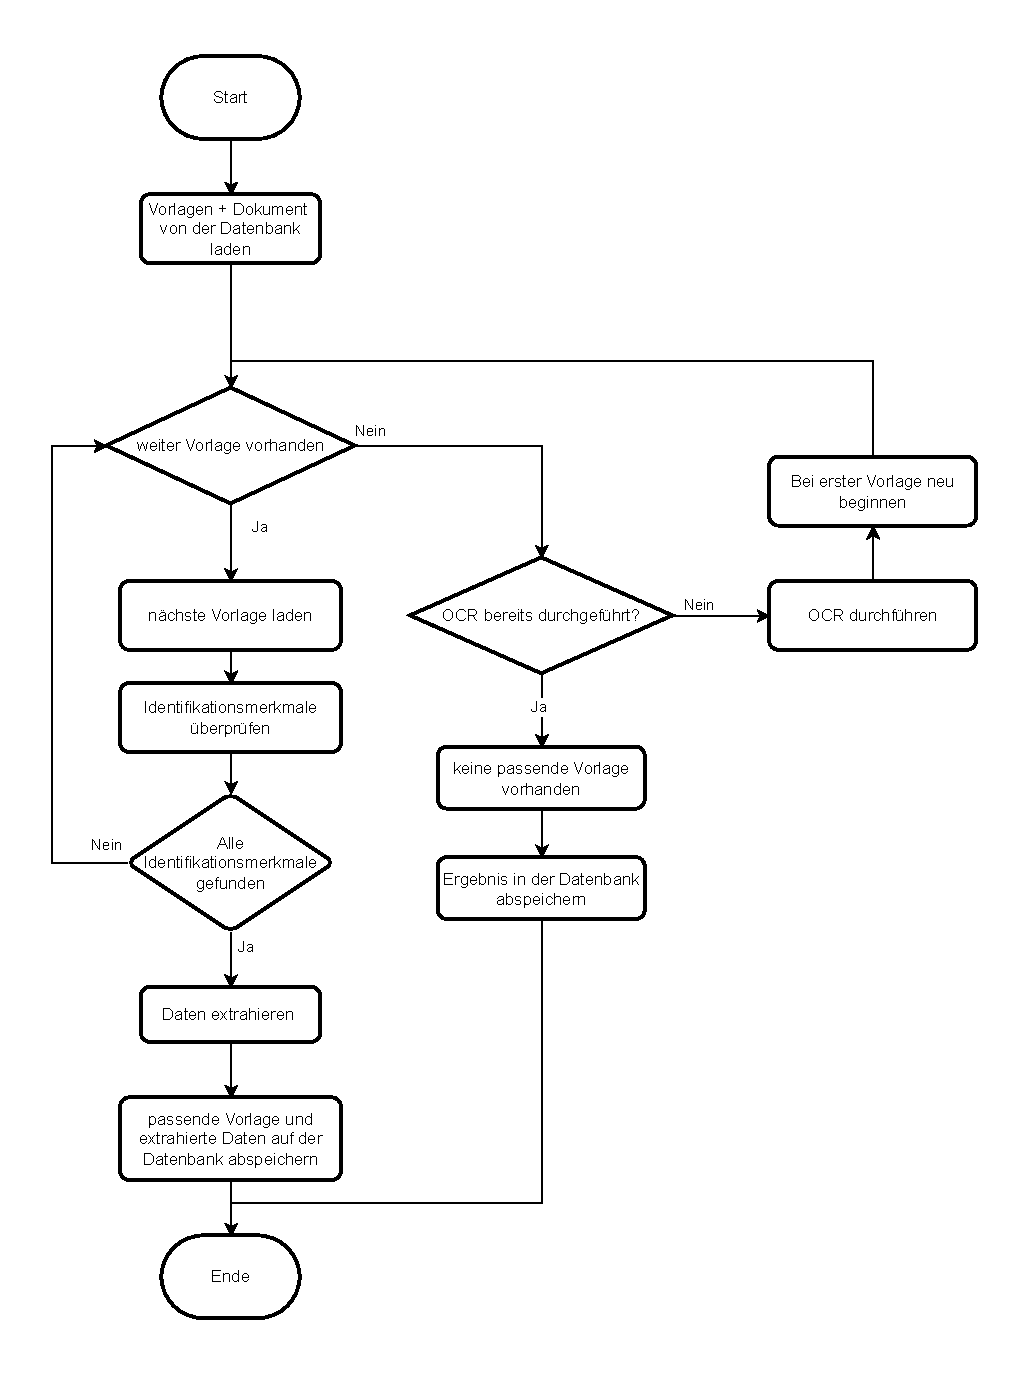
\includegraphics[width=\textwidth]{images/AuswertungBestehendesSystem.drawio.pdf}
	\caption{Ablaufdiagramm des bestehenden Systems}
	\label{fig:auswertung-bestehendes-system}
\end{figure}

Bei der Analyse neuer Dokumente vergleicht das System alle Vorlagen mit den Identifikationsmerkmalen. Bei einer Übereinstimmung extrahiert es die Daten aus den Suchfeldern und identifiziert den Dokumententyp sowie die Zusatzinformationen. Diese Typbestimmung steuert die nachfolgende Datenverarbeitung. Um Ressourcen zu schonen, versucht das System zunächst, eine Vorlage ohne \gls{OCR} zu finden. Scheitert dies, wendet es Tesseract-\gls{OCR} an, um den Text in Bildern zu erfassen, und wiederholt die Suche. Abbildung~\ref{fig:auswertung-bestehendes-system} visualisiert diesen Prozess. Kapitel \ref{subsec:tesseract-ocr} beschreibt das verwendete Tesseract \gls{OCR}-System detaillierter.

\subsection{Stärken und Schwächen}
\label{subsec:stärken-und-schwächen}

Das System überzeugt durch seinen einfachen Aufbau und arbeitet bei wenigen Vorlagen sehr effizient. Ein wesentlicher Vorteil liegt in der Fähigkeit, PDF-Dokumente mit bereits maschinenlesbarem Text ohne \gls{OCR} auszuwerten, was die Verarbeitungszeit erheblich reduziert. Erfahrungen zeigen, dass ein Großteil der zu verarbeitenden Dokumente im PDF-Format vorliegt. Allerdings enthalten viele dieser Dokumente trotz digitaler Erstellung Bilder mit relevantem Text, wodurch \gls{OCR} häufig notwendig bleibt.

Die sequenzielle Suche nach passenden Vorlagen führt zu einer linearen Skalierung der Laufzeit mit der Anzahl der definierten Vorlagen. Der wirtschaftlich bedeutendste Nachteil besteht im hohen manuellen Aufwand für die Definition einer Vorlage für jedes zu verarbeitende Dokumentenlayout. Dieser Aufwand steigt bei Dokumenten mit variabler Form, wie beispielsweise Rechnungen mit unterschiedlichen Positionsauflistungen, da das koordinatenbasierte System hier an seine Grenzen stößt.

Zudem eignet sich das System nicht für die zuverlässige Verarbeitung von Bildern mit schlechter Qualität, Verzerrungen oder Rotationen. Diese Einschränkungen in der Verarbeitbarkeit und mangelnde Flexibilität bei der Bildaufnahme erhöhen den manuellen Korrekturaufwand und erfordern erhöhte Sorgfalt bei der Dokumentenerfassung.

\section{Stand der Technik in der automatisierten Dokumentenverarbeitung}
\label{sec:stand-der-technik-in-der-automatisierten-dokumentenverarbeitung}

\subsection{Traditionelle Methoden der Dokumentenextraktion}
\label{subsec:traditionelle-Methoden-der-Dokumentenverarbeitung}

Historisch entwickelten Forscher*innen Ansätze zur Dokumentenextraktion hauptsächlich auf Basis von Vorlagen oder Regeln, die Kapitel \ref{subsubsec:regelbasierte-ansätze} detailliert erläutert \cite{YeYibin2018Auso, ChowdhuryGobindaG.1999Tmfi}. Grundlegend für viele dieser Ansätze ist der Fortschritt der \gls{OCR}-Technik, die Kapitel \ref{sec:optical-character-recognition-ocr} beschreibt.

Alternativ kommen auch NLP-basierte Ansätze zum Einsatz \cite{ChowdhuryGobindaG.1999Tmfi, MarinaiS.2005Annf}. Diese nutzen linguistische Analyse zur Informationsextraktion aus Texten, wobei Techniken wie Named Entity Recognition oder Part-of-Speech Tagging Anwendung finden. Herausforderungen bei der Implementierung NLP-basierter Dokumentenextraktionssysteme liegen vor allem in der Verarbeitung domänenspezifischer Sprache und der Kontextabhängigkeit von Textteilen.

Der Einsatz dieser Techniken kann Schwierigkeiten bezüglich der Skalierbarkeit auf große und diverse Dokumentmengen mit sich bringen \cite{ChowdhuryGobindaG.1999Tmfi, YeYibin2018Auso}. Die Vorteile dieser Methoden liegen hauptsächlich in der guten Leistung bei bekannten, konsistenten Dokumentenlayouts sowie der Interpretierbarkeit und relativ einfachen Nachvollziehbarkeit der Extraktionslogik. Zudem benötigen sie im Vergleich zu Machine-Learning-Ansätzen weniger Trainingsdaten \cite{ChowdhuryGobindaG.1999Tmfi, MarinaiS.2005Annf}.

\subsection{Deep-Learning-Ansätze}
\label{subsec:deep-learning-ansätze}

Deep Learning Ansätze revolutionierten in den letzten Jahren die Dokumentenverarbeitung. Im Gegensatz zu traditionellen regelbasierten Techniken lernen Deep-Learning-Modelle komplexe Muster direkt aus den Daten \cite{YangXiao2017LtES, XuYiheng2020LPoT}.

Entscheidend für diese Entwicklung war die Erforschung von Fully Convolutional Neural Networks (FCN) für die pixelweise Segmentierung von Dokumenten \cite{YangXiao2017LtES}. FCNs ermöglichen eine Ende-zu-Ende-Verarbeitung vom Eingabebild zur semantischen Segmentierung.

Innovative multimodale Ansätze wie MFCN\cite{YangXiao2017LtES} und LayoutLM\cite{XuYiheng2020LPoT} integrieren visuelle und textuelle Informationen in einem gemeinsamen Modell. Durch die Kombination von Bild- und Textmerkmalen erfassen diese Architekturen sowohl das Layout als auch den Inhalt von Dokumenten.

Die Vorteile von Deep-Learning-Ansätzen liegen vor allem in der automatischen Merkmalsextraktion, der verbesserten Verarbeitung komplexer Layouts und der gleichzeitigen Erkennung visueller und semantischer Klassen. Dies ermöglicht Spitzenleistungen bei verschiedenen Dokumentenverständnisaufgaben \cite{YangXiao2017LtES, XuYiheng2020LPoT}. Die Nachteile dieser Technik bestehen hauptsächlich im hohen Bedarf an annotierten Trainingsdaten sowie der Komplexität der Modelle und dem damit verbundenen Rechenaufwand beim Training \cite{YangXiao2017LtES, XuYiheng2020LPoT}.

\subsection{OCR-freie Document-Transformer}
\label{subsec:ocr-freie-document-transformer}

Die meisten aktuellen Methoden zur Umsetzung von Informationsextraktionsaufgaben nutzen \gls{OCR}-Methoden, um visuelle Dokumente in Text und teilweise auch in Layoutinformationen vorzuverarbeiten \cite{KimGeewook2022ODUT}. Dieser Vorverarbeitungsschritt bringt in der Regel einen hohen Rechenaufwand sowie eingeschränkte Flexibilität bei verschiedenen Sprachen mit sich. Zudem setzen sich Fehler, die beim \gls{OCR}-Prozess auftreten, im nachfolgenden Datenextraktionsschritt fort.

Um diese Probleme zu minimieren, entwickelten Forscher*innen mit \gls{DONUT} ein End-to-End-Modell, das das Eingangsbild direkt in strukturierte Daten verarbeitet \cite{KimGeewook2022ODUT}. Wie Abbildung \ref{fig:donut-comparison} zeigt, bringt dies sowohl Verbesserungen bezüglich des Ressourcenbedarfs als auch bei der Genauigkeit. Zusätzlich kann dieses Modell auch die Klassifizierung der Dokumente vornehmen, wodurch keine zusätzliche Komponente zur Klassifizierung notwendig wird.

\begin{figure}[htb]
	\centering
	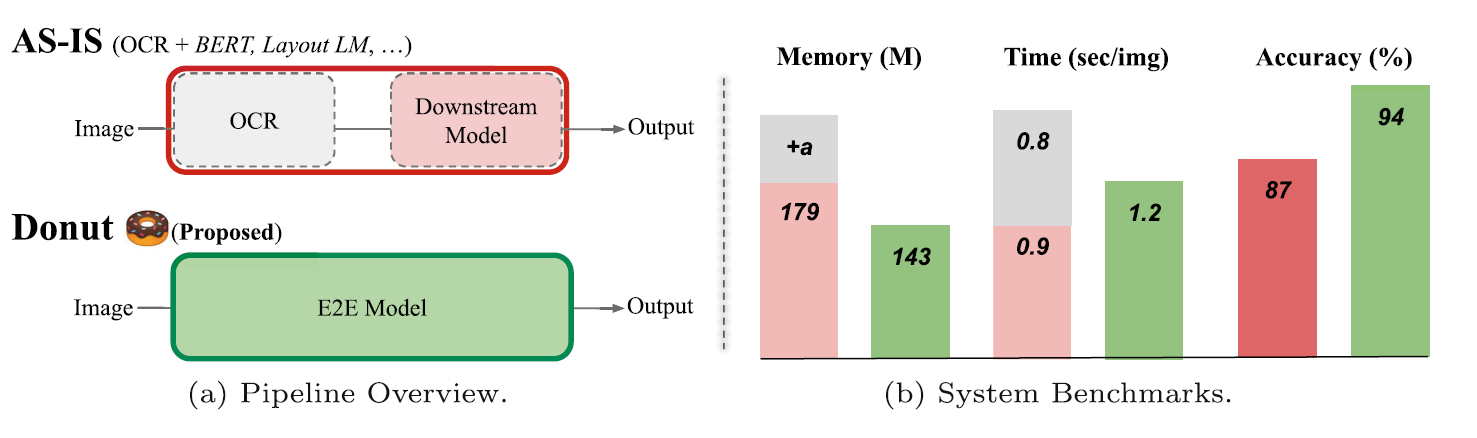
\includegraphics[width=\textwidth]{images/Donut_comparison.png}
	\caption{Vergleich des Ressourcenverbrauchs, der Performanz und Genauigkeit zwischen \gls{DONUT} und \gls{OCR}-basierten Ansätzen \cite{KimGeewook2022ODUT}}
	\label{fig:donut-comparison}
\end{figure}

\subsection{Language-Model-Prompting-basierte Document Information Extraction}
\label{subsec:language-model-basierte-document-information-extraction}

Ein weiterer vielversprechender Ansatz der Dokumentenextraktion nutzt die großen Fortschritte bei der Entwicklung von \glspl{LLM}. Forscher*innen bezeichnen die Methode als \gls{LMDX} und verwenden Prompting, um die Extraktion von Informationen aus visuell anspruchsvollen Dokumenten mithilfe von \glspl{LLM} zu ermöglichen \cite{PerotVincent2024LLMD}.

Der \gls{LMDX}-Ansatz, wie von \textcite{PerotVincent2024LLMD} beschrieben, besteht aus vier Hauptschritten:

\begin{enumerate}
	\item Chunking: Ein Algorithmus zerlegen das Dokument in kleinere Teile, die das \gls{LLM} verarbeiten kann.
	\item Prompt-Generierung: Für jeden Chunk wird ein Prompt erstellt, der den Dokumenteninhalt, eine Aufgabebeschreibung und das Zielschema enthält.
	\item \gls{LLM}-Inferenz: Das \gls{LLM} generiert Vervollständigungen basierend auf den Prompts.
	\item Dekodierung: Die \gls{LLM}-Ausgaben werden in strukturierte Entitäten und deren Positionen im Dokument umgewandelt.
\end{enumerate}

Ein wichtiges Element von \gls{LMDX} sind Koordinaten-Token, die das System verwendet, um Layoutinformationen auf textbasierte Weise an das \gls{LLM} zu übermitteln. Dadurch kann das \gls{LLM} auch das Layout des Dokuments berücksichtigen \cite{PerotVincent2024LLMD}. LLM-Prompting-basierte Parser eignen sich sowohl für die Datenextraktion als auch die Kategorisierung von Dokumenten. Die genaue Implementierung eines \gls{LMDX}-basierten Dokumentenverarbeitungssystems beschreibt Kapitel ... .

Die Vorteile von \gls{LMDX} liegen vor allem in seiner Flexibilität und der Unterstützung für die Extraktion von einzelnen, wiederholten und hierarchischen Entitäten. Außerdem ermöglicht es die Lokalisierung der extrahierten Entitäten im Dokument. Auch die Möglichkeit zur Zero-Shot-Extraktion ohne Trainingsprozess und die hohe Dateneffizienz bei der Anpassung an neue Dokumententypen sind besonders vorteilhaft für die Problemstellung. Die Nachteile bei der Verwendung hingegen liegen vor allem im relativ großen Rechenaufwand, den viele \glspl{LLM} verursachen. Zudem neigen \glspl{LLM} dazu, Informationen zu ``halluzinieren'', was die Zuverlässigkeit der Extraktion beeinträchtigen kann.

Tests und Benchmarks wie VRDU \cite{WangZilong2023VABf} und CORD \cite{park2019cord} zeigen, dass \gls{LMDX} den aktuellen Stand der Technik in verschiedenen Disziplinen der Dokumentenverarbeitung übertrifft oder zumindest eine robuste Lösung darstellt \cite{PerotVincent2024LLMD}. Die konkreten Werte im Vergleich mit anderen Modellen sind in der Tabelle \ref{tab:lmdx_cord_zero_shot_results} ersichtlich.

\begin{table}
	\centering
	\begin{tabular}{lcc}
		\hline
		Modell & Modalität & Micro-F1 \\
		\hline
		LLaVA-v1.5-13B & I & 5.97 \\
		GPT-4V$_\text{+Image}$ & I & 64.05 \\
		Gemini Pro$_\text{+Image}$ & I & 47.12 \\
		Gemini Pro$_\text{+OCR}$ & T & 59.57 \\
		PaLM 2-S$_\text{+OCR}$ & T & 55.85 \\
		GPT-3.5$_\text{+OCR}$ & T & 48.92 \\
		LMDX$_\text{PaLM 2-S}$ & T+L & \textbf{66.95} \\
		LMDX$_\text{Gemini Pro}$ & T+L & \underline{66.03} \\
		\hline
	\end{tabular}
	\caption{Micro-F1-Wert verschiedener Sprachmodell-basierten Dokumentenverarbeitungstechniken von Zero-Shot-Tests anhand des CORD \cite{park2019cord} Datensatzes, durchgeführt durch \textcite{PerotVincent2024LLMD} (T → Text, L → Layout, I → Image)}
	\label{tab:lmdx_cord_zero_shot_results}
\end{table}

\subsubsection{Verwendung multimodaler \glspl{LLM}}
\label{subsec:verwendung-multimodaler-llms}

Bei der Verarbeitung visueller Dokumente eignen sich besonders multimodale \glspl{LLM}, da diese die Bilder direkt verarbeiten können, ohne einen \gls{OCR}-Schritt und die damit verbundene Darstellung des Layouts in Textform zu benötigen.

Einige Beispiele für multimodale \glspl{LLM}, die für Dokumentenverständnis geeignet sind:

\begin{enumerate}
	\item DocLLM \cite{WangDongsheng2023DAlg}: Ein dokumentenzentriertes \gls{LLM}, das Informationsextraktion als Frage-Antwort-Aufgabe formuliert. Es ermöglicht Zero-Shot-Extraktion, hat jedoch Einschränkungen bei der Lokalisierung und der Extraktion hierarchischer Entitäten.
	\item LLaVA \cite{CaffagniDavide2024WHRG}: Ein multimodales Modell, das Bild- und Texteingaben verarbeiten kann. Obwohl es nicht speziell für Dokumentenverarbeitung entwickelt wurde, zeigt es Potenzial für dokumentenbezogene Aufgaben.
	\item GPT-4V \cite{openai_chatgpt} oder Claude \cite{anthropic_claude}: Diese fortgeschrittenen multimodalen Modelle von OpenAI bzw. Anthropic können Bild- und Texteingaben verarbeiten und zeigen vielversprechende Ergebnisse bei verschiedenen dokumentenbezogenen Aufgaben.
\end{enumerate}

Vorteile bei der Verwendung multimodaler \glspl{LLM} sind vor allem ihr ganzheitliches Verständnis von Text, Layout und anderen visuellen Elementen. Außerdem bieten sie, wie auch die textbasierten \glspl{LLM}, eine Flexibilität im Umgang mit verschiedenen Dokumentenlayouts sowie gute Zero-Shot-Fähigkeiten. Die Nachteile bei der Verwendung von multimodalen \glspl{LLM} sind weitgehend die gleichen wie bei der Verwendung von textbasierten \glspl{LLM}. Hinzu kommt jedoch, dass bei der Verwendung vieler multimodaler Modelle keine Lokalisierung der extrahierten Daten möglich ist.

\subsubsection{Behandlung von Halluzinationen}
\label{subsec:behandlung-von-halluzinationen}

Im Rahmen von \gls{LMDX} nannten \textcite{PerotVincent2024LLMD} auch Techniken zur Behandlung von Halluzinationen:

Es kann beispielsweise überprüft werden, ob die extrahierten Werte im Dokument enthalten sind. Ist dies nicht der Fall, muss es sich um eine Halluzination handeln, und der Wert wird verworfen. Dieser Ansatz bietet sich vor allem beim Einsatz von textbasierten \glspl{LLM} an, da diese Überprüfung anhand des im \gls{OCR}-Schritt extrahierten Rohtextes relativ einfach möglich ist. Eine zusätzliche, im selben Artikel genannte Methode verfolgt den Ansatz, mehrere Antworten (K Completions) für jeden Dokumentenchunk zu generieren. Die dadurch entstehenden Antworten können anschließend beispielsweise auf Basis eines Mehrheitsentscheids zusammengefügt werden, was eine Art ``Selbstkonsistenzprüfung'' darstellt. Zusätzlich sollte auch das im \gls{LMDX}-Prompt genutzte JSON-Schema verwendet werden, um das Ergebnis der Extraktion zu validieren, wodurch offensichtliche Halluzinationen oder Formatfehler erkannt werden können.

Weitere Methoden zur Reduzierung von Halluzinationen sind, das \gls{LLM} im Prompt explizit dazu zu ermutigen, bei geringer Konfidenz eher keinen Wert zurückzugeben \cite{BiswasAnjanava2024RoSD}. Zusätzlich beobachteten die Autor*innen in demselben Paper, dass \glspl{LLM} bei Bildern, in denen der Text zu stark rotiert ist, oft schlechtere Ergebnisse liefern. Deshalb ist es notwendig, die Bilder mit einem Deskewing-Algorithmus und eventuell auch anderen Bildverarbeitungsalgorithmen aufzubereiten, sodass der Text im Dokument möglichst gut lesbar ist, um damit die Zuverlässigkeit der Ergebnisse zu steigern.

\subsection{Bestehende Softwarelösungen}
\label{subsec:bestehende-softwarelösungen}

In den letzten Jahren hat der Einsatz automatischer Dokumentenverarbeitungssysteme in Unternehmen stark zugenommen \cite{PerotVincent2024LLMD}. Dies führte zur Entwicklung einer Vielzahl von Lösungen durch verschiedene Anbieter*innen. Die folgende Einteilung gängiger Lösungsansätze basiert auf einem Blogeintrag des Unternehmens Parsio \cite{parsio_pdf_extraction}.

\subsubsection{Vorlagenbasierte Parser}
\label{subsubsec:regelbasierte-ansätze}

Regelbasierte Parser verwenden hart codierte oder konfigurierbare Regeln zur Datenextraktion. Diese Regeln können auf regulären Ausdrücken, Textmustern, Layoutmustern oder Textpositionen basieren \cite{docparser_ruleBasedParsing}. Vorteile dieser Technologie sind die gute Performance und Genauigkeit der Ergebnisse. Die Nachteile liegen vor allem in dem hohen manuellen Aufwand, den das Definieren von Regeln erfordert. Dieser Lösungsweg ist daher nur sinnvoll, wenn Anwender*innen häufig Dokumente mit gleichen Eigenschaften und damit gleichen Regeln verarbeiten. Zudem ist es nicht möglich, alle Dokumententypen auf diese Art zu verarbeiten. Problematisch wäre beispielsweise in Fließtext enthaltene Information, da bei dieser Methode der Textinhalt nicht berücksichtigt wird. Beispiele für den Einsatz dieser Technologie sind der vorlagenbasierte Parser der Firma Docparser \cite{docparser_ruleBasedParsing} sowie entsprechende Parser der Firma Parsio \cite{parsio_pdf_extraction}.

\subsubsection{Zonal-OCR-Parser}
\label{subsubsec:zonal-ocr-parser}

Zonal-\gls{OCR}-Parser verwenden \gls{OCR}-Technik, um den Inhalt vordefinierter Bereiche eines Dokuments zu extrahieren. Wie bereits in Absatz \ref{subsec:architektur-und-funktionsweise} beschrieben, verwendet die bestehende Lösung der Firma Multidata diese Technik. Vorteile liegen vor allem in einer ressourceneffizienten Datenextraktion. Die Nachteile bestehen hauptsächlich in der mangelnden Flexibilität des Systems im Bezug auf Dokumente mit variablem Layout sowie dem hohen manuellen Aufwand, der vor allem durch die Notwendigkeit entsteht, die auszulesenden Bereiche zu definieren. Die Vor- und Nachteile der konkreten Lösung von Multidata sind in Absatz \ref{subsec:stärken-und-schwächen} genauer beschrieben. Ein weiteres Beispiel für den Einsatz dieser Technologie findet sich im Dokumentenverarbeitungssystem Docparser \cite{docparser_zonalOCR}.

\subsubsection{Machine-Learning-Modelle}
\label{subsubsec:vortrainierte-Modelle}

Machine-Learning-Modelle werden speziell für die Extraktion bestimmter Daten aus einer bestimmten Dokumentenart trainiert. Dies nehmen in der Regel entweder die Anbieter*innen des Dokumentenverarbeitungssystems vor oder entwickeln es konkret für einen Anwendungsfall. In beiden Fällen ist eine große Menge von Dokumenten mit den korrekten Ergebnissen erforderlich. Die benötigte Datenmenge können Entwickler*innen reduzieren, indem sie ein vortrainiertes Modell als Ausgangsbasis verwenden. Dieser Lösungsansatz liefert meist gute Ergebnisse für spezifische Anwendungsfälle. Außerdem können Anwender*innen diese Modelle ohne aufwendige manuelle Konfiguration verwenden. Der große Nachteil dieses Ansatzes ist jedoch die eingeschränkte Einsatzfähigkeit der Modelle. Zudem können Anwender*innen nur Dokumente sinnvoll verarbeiten, für die das Modell zuvor trainiert wurde. Auch das Hinzufügen eines neuen, zu extrahierenden Datenpunkts erfordert ein Neutraining des Modells. Da dabei sowohl Trainingsdaten vorbereitet als auch das Training selbst durchgeführt werden muss, bringt diese Änderung signifikante Kosten sowohl in Form von Personal- als auch Rechenaufwand mit sich. Ein Unternehmen, das Parser dieser Art anbietet, ist Parsio \cite{parsio_pdf_extraction}. Auch Google bietet sowohl vortrainierte Modelle als auch Werkzeuge zum Trainieren eigener Modelle im Rahmen seiner DocumentAI an \cite{google_documentAI}.

\subsubsection{Language-Modell-basierte Parser}
\label{subsubsec:llm-basierte-modelle}

Language-Modell\-basierte Parser verwenden in der Regel textbasierte \glspl{LLM} oder Question\-Answering-Modelle, um Informationen aus Dokumenten zu extrahieren. Dazu müssen bildbasierte Dokumente zunächst per \gls{OCR} in Text umgewandelt werden. Zur Umsetzung eines solchen Parsers können bekannte \glspl{LLM} wie GPT \cite{BrownTomB2020LMaF, openai_chatgpt} oder Claude \cite{anthropic_claude}, lokal hostbare \glspl{LLM} wie LLaMA \cite{TouvronHugo2023LOaE} oder auch Question\-Answering\-Modelle wie BERT \cite{DevlinJacob2019BPoD} verwendet werden.

Ein großer Vorteil dieser Technologie ist, dass das \gls{LLM} ein Verständnis von Kontext hat. Je nach verwendetem \gls{LLM} unterstützen diese oft auch viele verschiedene Sprachen. Zudem kommt diese Methode auch mit stark variablen Layouts aus und benötigt keine Vorlagen oder aufwendige manuelle Konfiguration. Zusätzlich bietet dieser Ansatz die Möglichkeit, die zu extrahierenden Daten jederzeit durch Änderung des Prompts anzupassen, ohne dass erneutes Training notwendig ist. Die Nachteile dieses Ansatzes liegen vor allem in seiner relativ ressourcenintensiven Natur sowie der Tendenz, Informationen zu halluzinieren. Dies können Entwickler*innen durch Ansätze, die in Absatz \ref{subsec:behandlung-von-halluzinationen} beschrieben werden, vermindern. Trotzdem ist eine manuelle Kontrolle der Ergebnisse zu empfehlen. Beispiele für den Einsatz dieser Methode sind der GPT-Parser der Firma Parsio \cite{parsio_pdf_extraction} oder die Box AI der Firma Box \cite{box_ai}.

\subsection{Bewertung der Anforderungserfüllung}
\label{subsec:bewertung-im-bezug-auf-die-anforderungen}

Im Bezug auf die in Absatz \ref{sec:problemstellung} beschriebenen Anforderungen bieten viele Parser zwar ausreichende Möglichkeiten, um Daten flexibel aus Dokumenten zu extrahieren. Die meisten Produkte, wie beispielsweise Box AI \cite{box_ai}, Parsios AI Parser \cite{parsio_pdf_extraction} sowie Google Document AI \cite{google_documentAI}, bieten jedoch nicht die Möglichkeit, die Systeme selbst zu hosten. Auch sind die Produkte einiger Unternehmen zu speziell auf eine bestimmte Branche und die damit verbundenen Anwendungsfälle zugeschnitten. Ein Beispiel dafür ist die automatische Rechnungserfassung von Finway \cite{finway_automatische_rechnungserfassung}, die sich auf Kreditorenprozesse spezialisiert hat.

Zudem bieten nur manche der Anbieter*innen Funktionen zur Klassifizierung der Dokumente an. Ein Beispiel dafür ist der Custom Document Classifier, den Google im Rahmen seiner Document AI anbietet \cite{google_documentAiCustomClassifier}. Dabei werden Werkzeuge zur Verfügung gestellt, die genutzt werden können, um Dokumentenklassifizierer zu trainieren, was aber auch bedeutet, dass das Hinzufügen einer neuen Dokumentenklasse zwingend ein erneutes Trainieren des Klassifizierungsmodells erfordert.

Ein Produkt, das alle Anforderungen erfüllt, ist Azure AI Document Intelligence von Microsoft \cite{microsoft_azureai_documentintelligence}. Dieses Produkt bietet sowohl die nötige Flexibilität beim Extrahieren der Daten von verschiedenen Dokumentenarten und können Anwender*innen außerdem in Form eines Docker-Containers selbst betreiben, sodass die Dokumente sowie die daraus extrahierten Daten nie die unternehmenseigenen Server verlassen müssen \cite{microsoft_azureai_documentintelligence_containers}. Aufgrund dessen wird dieses Produkt auch in den Tests in Absatz ... berücksichtigt.

\subsection{Aktuelle Ansätze zur Klassifizierung von Dokumenten}
\label{subsec:aktuelle-ansätze-zur-klassifizierung-von-dokumenten}

Liegen Dokumente unterschiedlichen Typs gemischt vor, ist es wichtig, dass das System diese klassifizieren und unterscheiden kann, da für verschiedene Dokumententypen oft auch unterschiedliche Daten extrahiert werden sollen. Wie in Absatz \ref{subsec:architektur-und-funktionsweise} beschrieben, nutzt das aktuelle System einen regelbasierten Ansatz, bei dem anhand der passenden Vorlage auch der Dokumententyp erkannt wird. Alternativ gibt es dazu auch noch andere Ansätze, welche im Folgenden beschrieben werden.

\subsubsection{Bildbasierte Klassifizierung}
\label{subsubsec:bild-basierte-klassifizieurng}

Bei bildbasierten Klassifizierungsverfahren wird versucht, die Bilder der Dokumente direkt zu klassifizieren. Wie von \textcite{HarleyAdamW2015EoDC} beschrieben, können dazu beispielsweise CNNs genutzt werden. Dabei können entweder holistische CNNs auf das ganze Bild angewandt oder ein Ensemble von regionsspezifischen CNNs verwendet werden. Letztere werden spezifisch für bestimmte Regionen des Dokuments trainiert und später auf diese Regionen angewandt. Die Resultate dieser Netze ergeben zusammen das Gesamtergebnis. Bei der Anwendung von CNNs zur Bildklassifizierung kann bei einer ausreichenden Menge von Trainingsdaten eine Genauigkeit von 85-90\% erwartet werden.

Problematisch bei diesem Ansatz im Bezug auf die Anforderungen ist, dass er eine große Menge von Trainingsdaten erfordert, welche aus Bildern und der dazugehörigen Kategorie bestehen. Dadurch wird die Flexibilität im Bezug auf die Möglichkeit, die Menge der Dokumententypen zu vergrößern beziehungsweise zu verkleinern, stark eingeschränkt, da dazu ein Neutrainieren des Modells sowie die nötigen Daten erforderlich sind.

\subsubsection{Textbasierte Klassifizierung}
\label{subsubsec:text-basierte-klassifizierung}

Für textbasierte Klassifizierung werden die Dokumente zunächst mittels \gls{OCR} in Text umgewandelt, um diesen Text anschließend mittels verschiedener Algorithmen zu klassifizieren. Dazu können beispielsweise Algorithmen wie Naïve Bayes, Decision Tree, Neural Network, Support Vector Machine oder hybride Ansätze verwendet werden \cite{dalal2011automatic, RasjidZulfanyErlisa2017PCaO, YangYiming1999Arot}. So wie bei den bildbasierten Klassifizierungsansätzen erfordern auch diese textbasierten Klassifizierungsalgorithmen Training, bei dem die Menge der Klassen bekannt sein muss. Dadurch ergeben sich die gleichen Probleme, wodurch auch dieser Ansatz die Anforderungen nur zum Teil erfüllt.

\subsubsection{Language-Model-basierte Klassifizierung}
\label{subsubsec:language-model-basierte-klassifizierung}

Ein weiterer Klassifizierungsansatz für Dokumente basiert auf Language Models. Dabei können sowohl textbasierte Modelle wie LLaMA oder BERT in sogenannten Zero-Shot-Aufgaben verwendet werden, um Text ohne erforderliches Training zu klassifizieren \cite{PuriRaul2019ZTCW, bert_as_classifier_without_fine_tuning}. Außerdem ist es auch möglich, multimodale LLMs zu verwenden, um die Bilder direkt zu klassifizieren \cite{LiJunnan2023BBLP, CaffagniDavide2024WHRG}. Hierbei gibt es verschiedene Techniken, wie beispielsweise den Prompt als Multiple-Choice-Aufgabe zu formulieren \cite{PuriRaul2019ZTCW}. Zudem ist es möglich, die Fill-Mask-Pipeline von BERT zu nutzen, um den Text zu klassifizieren \cite{bert_as_classifier_without_fine_tuning}.

\subsubsection{Vergleich der unterschiedlichen Methoden}
\label{subsubsec:vergleich-der-unterschiedlichen-methoden}

Bei der Wahl des Klassifizierungsverfahrens ist es wichtig, das verwendete Datenextraktionsverfahren in die Entscheidung mit einzubeziehen, um die Anzahl der benötigten Komponenten im System, die natürlich auch gehostet werden müssen, zu reduzieren. So bietet sich die auf textuellen \glspl{LLM} aufbauende Variante natürlich besonders in Kombination mit einer Datenextraktionstechnik an, die auf dem gleichen Modell basiert. Selbiges gilt auch für die Datenextraktionstechnik mit multimodalen \glspl{LLM}. Wird kein Language Model zur Datenextraktion verwendet, bieten sich auch bild- oder textbasierte Klassifizierungsverfahren an.

Zur Beschleunigung der Klassifizierung sowie der Verbesserung der Genauigkeit können auch regelbasierte Kategorisierungsmethoden verwendet werden, um leicht zu erkennende Fälle abzudecken. Hierzu könnte beispielsweise versucht werden, die Überschrift des Dokuments auszuwerten, sofern eine solche vorhanden ist. Dieser Ansatz wird in Absatz ... getestet.

\section{Herausforderungen}
\label{sec:herausforderungen-und-offene-probleme}

\subsection{Mehrsprachigkeit und kulturelle Unterschiede}
\label{subsec:mehrsprachigkeit-und-kulturelle-unterschiede}

Bei der Umsetzung von Dokumentenverarbeitungssystemen stellen Mehrsprachigkeit und kulturelle Unterschiede bedeutende Herausforderungen dar \cite{XuYiheng2020LPoT, SubramaniNishant2021ASoD}. Ein zentrales Problem sind \gls{OCR}-bezogene Schwierigkeiten, insbesondere bei weniger verbreiteten Sprachen oder Mischsprachen \cite{OlejniczakKrzysztof2023TDFA}.

Zur Bewältigung dieser Herausforderungen können verschiedene Ansätze genutzt werden:

\begin{enumerate}
	\item Systeme wie LayoutLM \cite{XuYiheng2020LPoT}, das für 12 verschiedene Sprachen trainiert wurde, gewährleisten eine breitere sprachliche Abdeckung. Allerdings bleiben viele Sprachen weiterhin unberücksichtigt.
	
	\item \gls{DONUT} \cite{KimGeewook2022ODUT} umgeht die sprachlichen Einschränkungen vieler \gls{OCR}-Systeme, indem es gänzlich ohne diese auskommt.
	
	\item Der \gls{LMDX}-Ansatz \cite{PerotVincent2024LLMD}, basierend auf multimodalen \glspl{LLM}, kann wie von \textcite{BiswasAnjanava2024RoSD} demonstriert, eingesetzt werden. Dies ist jedoch nur für Dokumentensprachen sinnvoll, die das verwendete Modell unterstützt.
\end{enumerate}

Eine weitere Herausforderung stellen kulturelle Unterschiede beim Layout der Dokumente dar \cite{KimGeewook2022ODUT}. Flexible Modellarchitekturen, wie von \textcite{KimGeewook2022ODUT} und \textcite{PerotVincent2024LLMD} vorgestellt, können verschiedene Layoutstile lernen und sich so besser an kulturelle Variationen anpassen.

Die Evaluierung und das Benchmarking mehrsprachiger Systeme erfordern repräsentative und diverse Datensätze, wie \textcite{SubramaniNishant2021ASoD} betonen. Zudem sind ethische Überlegungen zur Fairness und Vermeidung von Bias gegenüber bestimmten Sprachen oder Kulturen von großer Bedeutung. Alle betrachteten Sprachen oder kulturellen Layoutunterschiede sollten ausgewogen in Trainings- und Testdaten enthalten sein.

\subsection{Skalierbarkeit und Performanz}
\label{subsec:skalierbarkeit-und-performanz}

Die Skalierbarkeit und Performanz automatisierter Dokumentenverarbeitungssysteme stellen kritische Herausforderungen dar, insbesondere angesichts wachsender Datenmengen und komplexerer Verarbeitungsanforderungen. \textcite{PerotVincent2024LLMD} adressieren diese Problematik in ihrer Arbeit zu \gls{LMDX}, indem sie Ansätze zur effizienten Verarbeitung großer Dokumentmengen mit \glspl{LLM} vorstellen. Ihr Chunking-Algorithmus ermöglicht die Verarbeitung umfangreicher Dokumente, indem er diese in kleinere, vom \gls{LLM} verarbeitbare Teile zerlegt.

Ansätze wie \gls{DONUT} \cite{KimGeewook2022ODUT} erzielen eine bedeutende Performanzsteigerung, indem sie den rechenintensiven \gls{OCR}-Schritt einsparen.

Das Ressourcenmanagement bei rechenintensiven \gls{LLM}-basierten Ansätzen wie \gls{LMDX} \cite{PerotVincent2024LLMD} bleibt eine bedeutende Herausforderung. Die Entwicklung von Strategien zur effektiven Nutzung von Rechenressourcen, etwa durch verbesserte Parallelisierung, ist ein wichtiges Thema für die Zukunft automatisierter Dokumentenverarbeitungssysteme.

\subsection{Fehlerbehandlung und Kontrolle}
\label{subsec:fehlerbehandlung-und-kontrolle}

Für den Einsatz automatisierter Dokumentenverarbeitungssysteme ist die Behandlung von Fehlern ein essentielles Thema. Bei der Verwendung von Sprachmodellen ist es besonders wichtig, Halluzinationen zu minimieren. Ansätze dazu werden in Kapitel \ref{subsec:behandlung-von-halluzinationen} behandelt.

Zusätzlich ist es notwendig, die Ergebnisse der Informationsextraktion zu kontrollieren, um Fehler zu vermeiden, die wirtschaftlichen Schaden für Unternehmen, die das System verwenden, verursachen könnten. Das bestehende System von Multidata verwendet bereits einen zweistufigen Kontrollprozess:

\begin{enumerate}
	\item Ein automatischer Kontrollschritt prüft die extrahierten Daten auf ihre Plausibilität.
	
	\item Ein menschlicher Kontrollschritt, bei dem jedes verarbeitete Dokument von einem*einer Mitarbeiter*in überprüft und die Ergebnisse gegebenenfalls korrigiert werden.
\end{enumerate}

Nach umfangreichen Tests in der Praxis wäre es in Zukunft denkbar, diese Kontrolle auf kritische Ergebnisse oder besonders wichtige Dokumente zu beschränken, um den manuellen Aufwand zu minimieren.
\chapter{Lösungsdesign}
\label{cha:Lösungsdesign}
\chapter{Implementierung}
\label{cha:Implementierung}
\chapter{Evaluation}
\label{cha:Evaluation}
\chapter{Zusammenfassung und Ausblick}
\label{cha:Zusammenfassung und Ausblick}


%%%-----------------------------------------------------------------------------
\appendix                                                               % Anhang 
%%%-----------------------------------------------------------------------------

% \chapter{Technische Informationen}
\label{app:TechnischeInfos}

 % Technische Ergänzungen
% \chapter{Ergänzende Inhalte} % \chapter{Inhalt der CD-ROM/DVD}
\label{app:materials}


Auflistung der ergänzenden Materialien zu dieser Arbeit, die zur digitalen Archivierung an der 
Hochschule eingereicht wurden (als ZIP-Datei).

% Nur als Beispiel, die Struktur sollte man an die eigenen Bedürfnisse anpassen!

\section{PDF-Dateien}
\begin{FileList}{/}
\fitem{thesis.pdf} Finale Master-/Bachelorarbeit (Gesamtdokument)
\end{FileList}

\section{Mediendaten}
\begin{FileList}{/media}
\fitem{*.ai, *.pdf} Adobe Illustrator-Dateien
\fitem{*.jpg, *.png} Rasterbilder
\fitem{*.mp3} Audio-Dateien
\fitem{*.mp4} Video-Dateien
\end{FileList}


\section{Online-Quellen (PDF-Kopien)}
\begin{FileList}{/online-sources}
\fitem{Reliquienschrein-Wikipedia.pdf} {\backtrackerfalse\parencite{WikiReliquienschrein2023}}
\end{FileList}
 % Inhalt der CD-ROM/DVD
% \chapter{Fragebogen}
\label{app:Fragebogen}

 % Chronologische Liste der Änderungen
% \chapter{\latex-Quellcode}
\label{app:Quellcode}

 % Quelltext dieses Dokuments

%%%-----------------------------------------------------------------------------
\backmatter                          % Schlussteil (Quellenverzeichnis und dgl.)
%%%-----------------------------------------------------------------------------

\MakeBibliography % Quellenverzeichnis
\listoffigures % Abbildungsverzeichnis
\printglossary[type=\acronymtype,title=Abkürzungsverzeichnis]

%%%-----------------------------------------------------------------------------
% Messbox zur Druckkontrolle
%%%-----------------------------------------------------------------------------

% \chapter*{Messbox zur Druckkontrolle}



\begin{center}
{\Large --- Druckgröße kontrollieren! ---}

\bigskip

\calibrationbox{100}{50} % Angabe der Breite/Hoehe in mm

\bigskip

{\Large --- Diese Seite nach dem Druck entfernen! ---}

\end{center}



%%%-----------------------------------------------------------------------------
\end{document}
%%%-----------------------------------------------------------------------------
